% Provenance (never printed): see sources/outline_sources.md (Year 2: natural hazards and risks
% quantified --- recurrence, probabilistic hazard, slope stability, tsunamis, floods, warning).
% Terminology from the UN report A/71/644 (UNDRR); the 475-year convention from the USGS
% Earthquake Hazards 201 page; the ground-motion prediction equation of Boore, Joyner and Fumal
% (USGS Open-File Report 93-509); run-ups from the NOAA NCEI tsunami database; the 1999 Vargas
% debris flows from USGS Open-File Report 01-0144. Ledger rows in sources/ledger/book4.md;
% curves and numbers from figdata/bachelor-2/hazards.py and the Book 4 second-writer scratch
% calculator calc/ch28.py. Hazards are described and quantified physically only: no advice.
\chapter{Bahaya dan Risiko Geologi}\label{ch:b2:geological-hazards}

Bangunan yang dirancang untuk gerakan tanah yang terlampaui, secara rata-rata, sekali dalam 475 tahun memiliki
peluang satu banding sepuluh untuk mengalaminya selama umur lima puluh tahun. Kedua pernyataan itu adalah angka yang sama
yang dibaca dengan dua cara, dan berpindah di antara keduanya adalah pekerjaan sehari-hari ilmu bahaya. Bab ini
membangun alat-alatnya: probabilitas peristiwa langka, \omterm{def:b2:geological-hazards:psha}{kurva bahaya} suatu lokasi, kestabilan suatu
lereng, kecepatan dan \omterm{def:b2:geological-hazards:tsunami}{rayapan tsunami}, frekuensi banjir, serta fisika yang menentukan
seberapa banyak peringatan yang dapat diberikan oleh setiap bahaya.
% ledger: usgs:eh201-475

\begin{recall}
\textbf{Dari volume-volume sekolah}: bahaya alam, bencana alam, dan tanah longsor; kerentanan,
risiko, pencegahan, dan peta bahaya; tsunami; \omterm{def:b2:geological-hazards:return}{periode ulang} banjir, dan rumus peringkat
$T = (n + 1)/m$ untuk rekaman $n$ puncak tahunan. \textbf{Dari volume Tahun 1}: hukum
Gutenberg--Richter $\log_{10} N(\geq M) = a - bM$ dan nilai b-nya; momen seismik dan magnitudo
momen; tekanan fluida pori, tegangan efektif $\sigma' = \sigma - u$, dan kriteria keruntuhan
Coulomb $\tau = c' + \sigma' \tan\varphi'$. \textbf{Dari \cref{ch:b2:eruptive-styles}}: \omterm{def:b2:eruptive-styles:pdc}{arus densitas
piroklastik}, \omterm{def:b2:eruptive-styles:lahar}{lahar}, dan jatuhan \omterm{def:b2:eruptive-styles:tephra}{tefra}. \textbf{Dari buku-buku matematika}: distribusi Poisson dan
eksponensial, distribusi normal dan fungsi distribusinya $\Phi$.
\textbf{Dari volume Tahun 2 buku-buku fisika}: relasi dispersi gelombang gravitasi permukaan,
$\omega^2 = gk\tanh(kh)$.
\end{recall}

\section{Bahaya, keterpaparan, dan risiko}\label{sec:b2:geological-hazards:risk}

\begin{definition}[Bahaya geologi, keterpaparan, risiko bencana]\label{def:b2:geological-hazards:risk}
Yang disebut \emph{bahaya geologi}\index{bahaya geologi} adalah proses atau fenomena yang berasal dari
proses-proses internal Bumi --- gempa bumi, letusan, gerakan massa seperti
tanah longsor atau \omterm{def:b2:geological-hazards:slope}{aliran debris} --- dan dapat menimbulkan korban jiwa, cedera, kerusakan, atau gangguan. Bahaya itu
dicirikan oleh lokasinya, intensitas atau magnitudonya, serta frekuensi atau probabilitasnya. Yang disebut
\emph{keterpaparan}\index{keterpaparan (terhadap bahaya)} terhadap suatu bahaya adalah keadaan orang,
bangunan, infrastruktur, dan aset lain yang terletak di tempat yang dapat dijangkau bahaya itu, yang diukur dengan
jumlah atau nilainya. Yang disebut \emph{risiko bencana}\index{risiko bencana} adalah potensi kehilangan nyawa,
kesehatan, atau aset yang dapat terjadi dalam suatu periode tertentu, yang ditentukan secara probabilistik dari
bahaya, keterpaparan, dan kerentanan dari apa yang terpapar.
\end{definition}
% ledger: undrr:hazard, undrr:geological, undrr:exposure, undrr:disaster-risk, undrr:vulnerability

Terminologi internasional menggolongkan tsunami tersendiri: tsunami dipicu oleh gempa bumi dan peristiwa
geologi lain, lalu menjadi proses samudra dan melanda sebagai bahaya pesisir yang berkaitan dengan air.
Bab ini membahasnya bersama bahaya-bahaya lain, karena sumbernya bersifat geologi.
% ledger: undrr:geological

Definisi itu memuat suatu hasil kali. Jika peristiwa dengan intensitas $i$ terjadi dengan laju tahunan
$\lambda_i$, jika aset yang terpapar bernilai $E$, dan jika suatu peristiwa dengan intensitas $i$ menghancurkan
fraksi $V_i$ darinya (kerentanan, antara 0 dan 1), kerugian tahunan yang diharapkan adalah
\begin{equation}
L = \sum_i \lambda_i \, E \, V_i ,
\label{eq:b2:geological-hazards:loss}
\end{equation}
yang sering disingkat menjadi risiko = bahaya $\times$ \omterm{def:b2:geological-hazards:risk}{keterpaparan} $\times$ kerentanan. Risiko lenyap bila
salah satu faktornya lenyap: gunung api yang dahsyat di pulau yang kosong, kota yang padat di atas \omterm{def:b2:precambrian-earth:craton}{kraton} yang tenang, atau
bangunan yang tahan terhadap guncangan. Ilmu bahaya mengukur faktor pertama; gambar di bawah
menempatkannya di antara ketiganya.

\begin{omfigure}
\centering
\begin{tikzpicture}[font=\small]
\fill[omThm!14] (90:1.05) circle (1.55);
\fill[omDef!14] (210:1.05) circle (1.55);
\fill[black!8] (330:1.05) circle (1.55);
\begin{scope}
\clip (90:1.05) circle (1.55);
\clip (210:1.05) circle (1.55);
\fill[omThm!45!omDef!45] (330:1.05) circle (1.55);
\end{scope}
\draw[omThm, thick] (90:1.05) circle (1.55);
\draw[omDef, thick] (210:1.05) circle (1.55);
\draw[black!60, thick] (330:1.05) circle (1.55);
\node[align=center, anchor=south] at (0,2.65) {\textbf{bahaya} {\scriptsize (laju $\lambda_i$, intensitas)}};
\node[align=right, anchor=east] at (-2.55,-1.35) {\textbf{keterpaparan}\\[-1pt]{\scriptsize aset $E$}};
\node[align=left, anchor=west] at (2.55,-1.35) {\textbf{kerentanan}\\[-1pt]{\scriptsize fraksi yang hilang $V_i$}};
\node[align=center, font=\scriptsize\bfseries] at (0,0) {risiko};
\end{tikzpicture}
\par\smallskip{\small Tiga faktor \omterm{def:b2:geological-hazards:risk}{risiko bencana}. Kerugian yang diharapkan tidak nol hanya di tempat
ketiganya bertumpang tindih: bahaya yang menjangkau sesuatu yang terpapar dan dapat dirugikan.}
\end{omfigure}

\section{Probabilitas peristiwa langka}\label{sec:b2:geological-hazards:probability}

\begin{definition}[Periode ulang]\label{def:b2:geological-hazards:return}
Misalkan peristiwa-peristiwa sejenis --- banjir di atas suatu debit, gerakan tanah di atas suatu tingkat, gempa
bumi di atas suatu magnitudo --- terjadi dengan laju tahunan rata-rata $\lambda$. Yang disebut \emph{periode
ulang}\index{periode ulang} peristiwa itu adalah $T = 1/\lambda$: selang rata-rata antara dua peristiwa, dan
kebalikan laju tahunannya, bukan suatu jadwal.
\end{definition}
% ledger: usgs:eh201-475

\begin{definition}[Probabilitas pelampauan]\label{def:b2:geological-hazards:poisson}
Yang disebut \emph{probabilitas pelampauan}\index{probabilitas pelampauan} suatu tingkat dalam waktu paparan $t$
adalah probabilitas bahwa tingkat itu disamai atau dilampaui sedikitnya sekali selama $t$.
\end{definition}

\begin{proposition}[Model perulangan Poisson]\label{prop:b2:geological-hazards:poisson}
Misalkan peristiwa-peristiwa terjadi satu per satu\index{model perulangan Poisson}, saling bebas satu sama
lain dan bebas dari waktu yang telah berlalu, dengan laju rata-rata konstan $\lambda = 1/T$. Maka banyaknya $N$
peristiwa dalam waktu $t$ mengikuti distribusi Poisson dengan rata-rata $\lambda t$; \omterm{def:b2:geological-hazards:poisson}{probabilitas
pelampauan} dalam $t$ adalah
\begin{equation}
P(t) = 1 - e^{-t/T};
\label{eq:b2:geological-hazards:poisson}
\end{equation}
dan selang antara peristiwa-peristiwa yang berurutan mengikuti distribusi eksponensial dengan rata-rata $T$.
\end{proposition}

\begin{proof}
Misalkan $P_k(t)$ probabilitas terjadinya $k$ peristiwa dalam $[0, t]$. Dalam selang pendek $\mathrm{d}t$ suatu
peristiwa terjadi dengan probabilitas $\lambda\,\mathrm{d}t$, tidak bergantung pada masa lalu, dan dua peristiwa dengan
probabilitas berorde lebih tinggi. Karena itu $P_0(t + \mathrm{d}t) = P_0(t)(1 - \lambda\,\mathrm{d}t)$, yaitu
$P_0' = -\lambda P_0$ dengan $P_0(0) = 1$: $P_0(t) = e^{-\lambda t}$, dan $P(t) = 1 - P_0(t)$. Dengan
cara yang sama $P_k' = \lambda(P_{k-1} - P_k)$ untuk $k \geq 1$, yang diselesaikan dengan induksi:
$P_k(t) = (\lambda t)^k e^{-\lambda t}/k!$, distribusi Poisson dengan rata-rata $\lambda t$. Bila dimulai pada
suatu peristiwa, argumen yang sama memberikan probabilitas bahwa peristiwa berikutnya datang lebih lambat daripada $t$:
$e^{-\lambda t}$, fungsi kesintasan distribusi eksponensial, yang rata-ratanya
$\int_0^\infty e^{-\lambda t}\,\mathrm{d}t = 1/\lambda = T$.
\end{proof}

Dua akibatnya dipakai di mana-mana. Untuk probabilitas $p$ dalam waktu paparan $t$, \omterm{def:b2:geological-hazards:return}{periode
ulangnya} adalah $T = -t/\ln(1 - p)$: \qty{10}{\percent} dalam 50 tahun memberikan $T = 50/0.10536 =
474.6$ tahun, yaitu gerakan ``475 tahun'' dalam peraturan bangunan, dan \qty{2}{\percent} dalam 50 tahun
memberikan 2475 tahun. Dan bila $t \ll T$, $P \approx t/T$: laju itu dapat dibaca sebagai
probabilitas per tahun. Sebaliknya, selama satu \omterm{def:b2:geological-hazards:return}{periode ulang} penuh probabilitasnya adalah $1 - e^{-1} =
\qty{63}{\percent}$, bukan 1. Gambar di bawah (kiri) menggambarkan \eqref{eq:b2:geological-hazards:poisson}
untuk tiga \omterm{def:b2:geological-hazards:return}{periode ulang}.
% ledger: usgs:eh201-475
% values: T 474.561 and 2474.92 years; P(50|475) 0.0999 (hazards.py numbers)

Apakah model itu benar? Katalog global gempa bumi bermagnitudo sedikitnya 7 memuat 696 peristiwa
dari 1976 sampai 2025, yaitu 695 selang dengan rata-rata 26.2 hari. Jika gempa-gempa itu merupakan proses Poisson,
fraksi selang yang lebih panjang daripada $t$ akan sebesar $e^{-t/26.2}$, suatu garis lurus pada sumbu
logaritmik. Gambar di bawah (kanan) menunjukkan bahwa hampir demikian: \qty{30.4}{\percent} selang
lebih panjang daripada 30 hari, dibandingkan dengan \qty{31.8}{\percent} menurut model, dan simpangan baku
selang-selang itu 1.07 kali rata-ratanya, dibandingkan dengan tepat 1. Cacatnya ada pada selang yang pendek: 36 pasang
jatuh pada hari yang sama, gempa susulan dan gempa kembar yang tidak akan berkerumun dalam proses tanpa ingatan. Karena itu peta
bahaya membuang peristiwa-peristiwa yang bergantung dari katalog, yaitu memilah gugusannya (\textit{declustering}), sehingga
gempa-gempa utama yang tersisa dapat diperlakukan sebagai proses Poisson; lajunya menurut magnitudo berasal dari
hukum Gutenberg--Richter.
% ledger: data:usgs-comcat, usgs:eh201-poisson
% values: m7_events 696, mean 26.2245 d, cv 1.06891, same-day 36, frac>30 d 0.303597 vs 0.318552

\begin{omfigure}
\centering
\begin{minipage}[b]{0.49\linewidth}\centering
\begin{tikzpicture}
\begin{axis}[omrecord, width=0.96\linewidth, height=5.2cm, xmin=0, xmax=200, ymin=0, ymax=1,
  xlabel={waktu paparan $t$ (tahun)}, ylabel={probabilitas pelampauan},
  tick label style={font=\scriptsize}, label style={font=\small},
  xtick={0,50,100,150,200}, ytick={0,0.2,...,1}]
% computed in figdata/bachelor-2/hazards.py part poisson
\addplot[omThm, line width=1pt] table[x=t_yr, y=P50] {figdata/out/bachelor-2-hazards-poisson.dat};
\addplot[omDef, line width=1pt] table[x=t_yr, y=P475] {figdata/out/bachelor-2-hazards-poisson.dat};
\addplot[black!70, line width=1pt, densely dashed] table[x=t_yr, y=P2475] {figdata/out/bachelor-2-hazards-poisson.dat};
\draw[black!50, densely dotted] (axis cs:50,0) -- (axis cs:50,1);
\fill[omDef] (axis cs:50,0.1) circle (1.8pt);
\node[font=\scriptsize, text=omThm, anchor=west] at (axis cs:62,0.86) {$T = 50$};
\node[font=\scriptsize, text=omDef, anchor=west] at (axis cs:120,0.34) {$T = 475$};
\node[font=\scriptsize, text=black!70, anchor=west] at (axis cs:120,0.12) {$T = 2475$};
\node[font=\scriptsize, anchor=west, text=omDef] at (axis cs:52,0.2) {\qty{10}{\percent}};
\end{axis}
\end{tikzpicture}
\end{minipage}\hfill
\begin{minipage}[b]{0.49\linewidth}\centering
\begin{tikzpicture}
\begin{axis}[omrecord, width=0.93\linewidth, height=5.2cm, xmin=0, xmax=120, ymode=log,
  ymin=0.008, ymax=1.1, xlabel={selang $t$ (hari)}, ylabel={fraksi selang $> t$},
  tick label style={font=\scriptsize}, label style={font=\small}, xtick={0,30,60,90,120},
  legend style={at={(0.03,0.03)}, anchor=south west, font=\scriptsize, draw=black!30},
  legend cell align=left]
% computed in figdata/bachelor-2/hazards.py part survival; ledger: data:usgs-comcat
\addplot[omThm, only marks, mark=*, mark size=1.2pt] table[x=t_day, y=observed] {figdata/out/bachelor-2-hazards-survival.dat};
\addlegendentry{$M \geq 7$, 1976--2025}
\addplot[black, line width=0.9pt] table[x=t_day, y=poisson] {figdata/out/bachelor-2-hazards-survival.dat};
\addlegendentry{Poisson, rata-rata 26.2 hari}
\end{axis}
\end{tikzpicture}
\end{minipage}
\par\smallskip{\small Kiri: probabilitas sedikitnya satu peristiwa dalam waktu paparan $t$ untuk
\omterm{def:b2:geological-hazards:return}{periode ulang} 50, 475, dan 2475 tahun; peristiwa 475 tahun berpeluang \qty{10}{\percent} dalam 50
tahun. Kanan: selang antara 696 gempa bumi bermagnitudo sedikitnya 7 dalam katalog
global 1976--2025, dibandingkan dengan hukum eksponensial proses Poisson dengan laju yang sama. Data:
USGS ANSS Comprehensive Catalog.}
\end{omfigure}

\section{Bahaya seismik}\label{sec:b2:geological-hazards:seismic}

\begin{definition}[Analisis bahaya seismik probabilistik, persamaan prediksi gerakan tanah, percepatan tanah puncak, kurva bahaya]\label{def:b2:geological-hazards:psha}
Yang disebut \emph{percepatan tanah puncak}\index{percepatan tanah puncak} (PGA) di suatu lokasi adalah percepatan
horizontal mutlak terbesar tanah selama gempa bumi, biasanya dinyatakan sebagai
fraksi $g$. Yang disebut \emph{persamaan prediksi gerakan tanah}\index{persamaan prediksi gerakan tanah}
(GMPE) memberikan distribusi probabilitas suatu ukuran guncangan seperti PGA di suatu
lokasi --- median dan sebaran --- sebagai fungsi magnitudo, jarak ke sumber,
dan kondisi tanah. Yang disebut \emph{analisis bahaya seismik probabilistik}\index{analisis bahaya seismik probabilistik}
(PSHA) menggabungkan semua gempa bumi yang dapat memengaruhi suatu lokasi, beserta
laju dan jaraknya, dengan suatu GMPE, untuk memberikan laju tahunan terlampauinya setiap tingkat guncangan.
Kurva laju itu terhadap tingkatnya adalah \emph{kurva
bahaya}\index{kurva bahaya} lokasi tersebut.
\end{definition}
% ledger: usgs:eh201-pga, usgs:eh201-475

PGA adalah apa yang dialami oleh suatu partikel tanah. Bangunan menanggapi bagian
gerakan di sekitar periode alaminya sendiri, dan peraturan bangunan juga memetakan tanggapan itu, yaitu percepatan spektral;
PGA membuat penalaran tetap sederhana dan dipakai di sini.
% ledger: usgs:eh201-pga

\begin{method}[Analisis bahaya seismik probabilistik]\label{met:b2:geological-hazards:psha}
\begin{enumerate}
  \item \textbf{Sumber.} Petakan sesar dan zona sumber di sekitar lokasi, serta jarak $d$ masing-masing
        ke lokasi itu.
  \item \textbf{Perulangan.} Untuk setiap sumber, ambillah laju tahunan gempa bumi menurut magnitudo
        dari hukum Gutenberg--Richter yang dipotong pada magnitudo maksimum $M_{\max}$:
        $N(\geq m) = 10^{a - bm} - 10^{a - bM_{\max}}$, mulai dari magnitudo minimum $M_{\min}$.
        Potonglah rentang itu menjadi irisan-irisan dengan laju $\nu_j$ di sekitar magnitudo $m_j$.
  \item \textbf{Gerakan tanah.} Dari GMPE, ambillah median $\mu_j = \log_{10}\mathrm{PGA}$ dan
        sebaran $\sigma$ untuk setiap irisan; probabilitas bahwa PGA melampaui $a$ adalah
        $1 - \Phi\bigl((\log_{10} a - \mu_j)/\sigma\bigr)$.
  \item \textbf{Jumlah.} Laju tahunan pelampauan $a$ adalah $\lambda(a) = \sum_j \nu_j
        \bigl[1 - \Phi\bigl((\log_{10} a - \mu_j)/\sigma\bigr)\bigr]$, yang dijumlahkan atas semua sumber.
  \item \textbf{Baca.} PGA dengan \omterm{def:b2:geological-hazards:poisson}{probabilitas pelampauan} $p$ dalam $t$ tahun adalah tingkat ketika
        $\lambda(a) = -\ln(1 - p)/t$: \num{2.107e-3} per tahun untuk \qty{10}{\percent} dalam 50 tahun.
\end{enumerate}
\end{method}

GMPE yang dipakai dalam bab ini adalah GMPE Boore, Joyner, dan Fumal, yang dicocokkan dengan 271 rekaman dari 20
gempa bumi di Amerika Utara bagian barat: untuk komponen horizontal acak, dalam satuan $g$,
\begin{equation}
\log_{10}\mathrm{PGA} = -0.105 + 0.229\,(M - 6) - 0.778\log_{10} r + 0.162\,G_B + 0.251\,G_C,
\qquad r = \sqrt{d^2 + 5.57^2},
\label{eq:b2:geological-hazards:gmpe}
\end{equation}
dengan $M$ magnitudo momen, $d$ jarak dalam kilometer ke proyeksi permukaan
retakan, dan sebaran $\sigma = 0.230$ di sekitar median. Persamaan itu berlaku untuk $5.0 \leq M \leq 7.7$ dan $d
\leq \qty{100}{km}$. Konstanta \qty{5.57}{km} adalah kedalaman fiktif yang dicocokkan oleh regresi,
yang menjaga gerakan tetap berhingga di atas sumber. Magnitudo 6 pada \qty{15}{km} memberikan median
\qty{0.091}{g}, magnitudo 7.5 \qty{0.200}{g}; satu simpangan baku mengalikan atau membagi
median dengan $10^{0.230} = 1.70$.
% ledger: bjf93:pga, bjf97:pga-ln
% values: M6@15 km 0.0908 g, M7.5@15 km 0.2003 g (hazards.py numbers)

Suku $G_B$ dan $G_C$ membawa efek lokasi. Lokasi digolongkan menurut kecepatan rata-rata gelombang geser
di \qty{30}{m} teratasnya: kelas A di atas \qty{750}{m.s^{-1}} ($G_B = G_C = 0$), kelas B dari
360 sampai \qty{750}{m.s^{-1}} ($G_B = 1$), dan kelas C dari 180 sampai \qty{360}{m.s^{-1}} ($G_C = 1$). Tanah
lunak mengalikan gerakan batuan dengan $10^{0.162} = 1.45$ pada kelas B dan $10^{0.251} = 1.78$ pada kelas
C: gelombang yang memasuki bahan yang lebih lambat menjadi lambat, memendek, dan amplitudonya membesar, dan lapisan lunak atau
cekungan berisi sedimen dapat beresonansi dan memerangkapnya.
% ledger: bjf93:pga

Gambar di bawah menerapkan metode itu pada satu zona sumber yang berjarak \qty{15}{km} dari lokasi batuan, dengan $a
= 4.0$, $b = 1.0$, $M_{\min} = 5$, dan $M_{\max} = 7.5$: sekitar 0.1 gempa bumi bermagnitudo 5 atau
lebih per tahun. Pada PGA kecil kurva itu mendekati laju tersebut, karena setiap gempa bumi melampaui tingkat
yang lemah. PGA \qty{10}{\percent}-dalam-50-tahun adalah \qty{0.22}{g}. Seandainya setiap gempa bumi menghasilkan
tepat mediannya, laju yang sama akan tercapai pada \qty{0.13}{g}, dan tidak ada tingkat di atas median
gempa bumi terbesar, \qty{0.20}{g}, yang dapat terlampaui. Sebaran mendominasi tingkat-tingkat
yang langka: gerakan 475 tahun sebagian besar berasal dari gempa bumi sedang yang mengguncang lebih keras daripada
mediannya.
% values: psha_rate_m5 0.0997, psha_pga475 0.220894, psha_pga475_median 0.125607, median M7.5 0.2003 (hazards.py numbers)

\begin{omfigure}
\centering
\begin{tikzpicture}
\begin{axis}[omrecord, width=0.8\linewidth, height=5.6cm, xmode=log, ymode=log, xmin=0.01,
  xmax=2, ymin=1e-6, ymax=0.3, xlabel={percepatan tanah puncak (\unit{g})},
  ylabel={laju tahunan pelampauan}, unbounded coords=jump,
  tick label style={font=\scriptsize}, label style={font=\small},
  xtick={0.01,0.03,0.1,0.3,1}, xticklabels={0.01,0.03,0.1,0.3,1},
  legend style={at={(0.03,0.03)}, anchor=south west, font=\scriptsize, draw=black!30},
  legend cell align=left]
% computed in figdata/bachelor-2/hazards.py part psha; ledger: bjf93:pga
\addplot[omThm, line width=1.2pt] table[x=pga_g, y=rate] {figdata/out/bachelor-2-hazards-psha.dat};
\addlegendentry{dengan sebaran GMPE}
\addplot[black!60, line width=1pt, densely dashed] table[x=pga_g, y=rate_median] {figdata/out/bachelor-2-hazards-psha.dat};
\addlegendentry{median saja}
\draw[omDef, densely dotted, thick] (axis cs:0.01,2.107e-3) -- (axis cs:2,2.107e-3);
\draw[omDef, densely dotted, thick] (axis cs:0.2209,1e-6) -- (axis cs:0.2209,2.107e-3);
\node[font=\scriptsize, text=omDef, anchor=south east] at (axis cs:2,2.107e-3) {\qty{10}{\percent} dalam 50 tahun};
\node[font=\scriptsize, text=omDef, anchor=west] at (axis cs:0.235,2e-5) {\qty{0.22}{g}};
\end{axis}
\end{tikzpicture}
\par\smallskip{\small \omterm{def:b2:geological-hazards:psha}{Kurva bahaya}: laju tahunan terlampauinya setiap tingkat oleh PGA di suatu lokasi batuan,
untuk satu zona sumber pada \qty{15}{km} (perulangan Gutenberg--Richter terpotong, $b = 1$,
magnitudo 5 sampai 7.5) dan GMPE Boore, Joyner, dan Fumal. Garis-garis titik membaca tingkat
\qty{10}{\percent}-dalam-50-tahun. Tanpa sebaran (putus-putus) kurva itu berhenti pada median
gerakan gempa bumi terbesar.}
\end{omfigure}

\section{Bahaya gunung api}\label{sec:b2:geological-hazards:volcanic}

Gunung api mengancam melalui beberapa proses sekaligus, masing-masing dengan jangkauannya sendiri: \omterm{def:b2:eruptive-styles:tephra}{tefra} jatuh jauh
searah angin, \omterm{def:b2:eruptive-styles:pdc}{arus densitas piroklastik} dan \omterm{def:b2:eruptive-styles:lahar}{lahar} mengikuti lembah, aliran lava maju dengan lambat
(\cref{ch:b2:eruptive-styles}). Peta bahayanya menggambar satu zona untuk masing-masing, dari endapan letusan-letusan
masa lalu dan dari model aliran dan jatuhan. Probabilitasnya dibangun secara berbeda dari probabilitas
gempa bumi, karena gunung api yang mulai aktif kembali bukanlah proses yang stasioner. Suatu pohon kejadian mengarah
dari peningkatan aktivitas ke hasil-hasil melalui cabang-cabang, masing-masing dari suatu peristiwa prasyarat yang perlu ke hasil yang lebih
spesifik --- peningkatan aktivitas, magmatik atau tidak; letusan atau tidak; eksplosif atau efusif; \omterm{def:b2:eruptive-styles:pdc}{aliran piroklastik}
mencapai suatu lembah tertentu atau tidak. Probabilitas suatu hasil adalah hasil kali probabilitas
bersyarat di sepanjang cabangnya. Dengan $M$ peningkatan aktivitas magmatik, $E$ letusan, $X$ \omterm{def:b2:eruptive-styles:regimes}{erupsi
eksplosif}, dan $V$ aliran di lembah itu,
\begin{equation*}
P(V) = P(M) \, P(E \mid M) \, P(X \mid E) \, P(V \mid X),
\end{equation*}
masing-masing faktor diperkirakan dari masa lalu gunung api itu, dari gunung api yang sebanding, atau dari model, lalu diperbarui dengan
teorema Bayes seiring datangnya data pemantauan baru (\cref{exo:b2:geological-hazards:8}).
% ledger: nh02:event-tree

\section{Tanah longsor}\label{sec:b2:geological-hazards:landslides}

Suatu lereng tetap berdiri selama kekuatan bahannya, di sepanjang permukaan mana pun yang dapat menjadi tempatnya meluncur,
melampaui tegangan yang diberikan gravitasi di sana. Kekuatan itu adalah kriteria Coulomb dari volume
Tahun 1, yang ditulis dalam tegangan efektif: air di dalam pori memikul sebagian beban normal dan
menurunkan gesekan.

\begin{definition}[Faktor keamanan, aliran debris]\label{def:b2:geological-hazards:slope}
Yang disebut \emph{faktor keamanan}\index{faktor keamanan} $F$ suatu lereng di sepanjang bidang gelincir potensial
adalah perbandingan kekuatan geser yang tersedia pada bidang itu terhadap tegangan geser yang diperlukan untuk
kesetimbangan. Lereng itu stabil untuk $F > 1$ dan runtuh ketika $F$ turun menjadi 1. Yang disebut \emph{aliran
debris}\index{aliran debris} adalah aliran cepat lumpur, pasir, kerikil, bongkah, dan kayu yang jenuh air
yang bergerak menuruni suatu alur sebagai satu massa padat, dengan butir-butir yang memikul sebagian besar beratnya, lalu menyebar
di atas kipas di mulut alur itu.
\end{definition}

\begin{proposition}[Lereng tak berhingga]\label{prop:b2:geological-hazards:infinite-slope}
Suatu lapisan tanah dengan berat satuan $\gamma$ dan tebal $z$, yang diukur secara vertikal, terletak di atas bidang
gelincir yang sejajar dengan permukaan tanah dengan sudut $\beta$; kekuatannya adalah $c'$ dan $\varphi'$, dan
tekanan pori pada bidang itu adalah $u = r_u \gamma z$. Jika lapisan itu cukup panjang sehingga ujung-ujungnya dapat
diabaikan,
\begin{equation}
F = \frac{c' + \gamma z\,(\cos^2\beta - r_u)\tan\varphi'}{\gamma z \sin\beta\cos\beta}.
\label{eq:b2:geological-hazards:infinite-slope}
\end{equation}
Untuk lapisan yang kering dan tak berkohesi, $F = \tan\varphi'/\tan\beta$: lapisan itu tetap berdiri sampai $\beta = \varphi'$.
\end{proposition}

\begin{proof}
Ambillah suatu kolom lapisan dengan lebar horizontal $b$. Beratnya $W = \gamma z b$ per satuan panjang
melintang lereng, dan alasnya, yang sejajar dengan permukaan, memiliki panjang $b/\cos\beta$. Gaya-gaya pada
kedua sisinya sama besar dan berlawanan arah dalam lereng tak berhingga, sehingga saling meniadakan. Dengan menguraikan $W$ tegak lurus dan
sejajar dengan alas, lalu membaginya dengan panjang alas, tegangan normal dan geser pada alas adalah
$\sigma = \gamma z\cos^2\beta$ dan $\tau = \gamma z \sin\beta\cos\beta$. Tegangan normal
efektifnya $\sigma' = \sigma - u = \gamma z(\cos^2\beta - r_u)$, kekuatan yang tersedia $c' +
\sigma'\tan\varphi'$, dan $F$ adalah perbandingan keduanya. Dengan $c' = 0$ dan $r_u = 0$, $F = \cos^2\beta
\tan\varphi'/(\sin\beta\cos\beta) = \tan\varphi'/\tan\beta$.
\end{proof}

\begin{omfigure}
\centering
\begin{minipage}[b]{0.49\linewidth}\centering
\begin{tikzpicture}[scale=0.82, font=\scriptsize]
\def\t{0.57735}
\fill[black!10] (0,-1) -- (5.6,{5.6*\t-1}) -- (5.6,-1.6) -- (0,-1.6) -- cycle;
\fill[omThm!12] (0,0) -- (5.6,{5.6*\t}) -- (5.6,{5.6*\t-1}) -- (0,-1) -- cycle;
\draw[thick] (0,0) -- (5.6,{5.6*\t});
\draw[omDef, densely dashed] (0,-0.4) -- (5.6,{5.6*\t-0.4});
\draw[omThm, very thick] (0,-1) -- (5.6,{5.6*\t-1});
\fill[white, opacity=0.55] (2.4,{2.4*\t}) -- (3.2,{3.2*\t}) -- (3.2,{3.2*\t-1}) -- (2.4,{2.4*\t-1}) -- cycle;
\draw[black!75] (2.4,{2.4*\t}) -- (3.2,{3.2*\t}) -- (3.2,{3.2*\t-1}) -- (2.4,{2.4*\t-1}) -- cycle;
\draw[->, thick] (2.8,{2.8*\t-0.3}) -- (2.8,{2.8*\t-1.35}) node[below] {$W$};
\draw[<->] (4.6,{4.6*\t-1}) -- (4.6,{4.6*\t}) node[midway, right] {$z$};
\draw[black!60] (0.25,-1) -- (1.45,-1);
\draw[black!60] (1.25,-1) arc (0:30:1.0);
\node at (1.55,-0.78) {$\beta$};
\node[omDef, anchor=north, rotate=30, inner sep=1.5pt] at (1.15,{1.15*\t-0.4}) {muka air tanah};
\node[omThm, anchor=north, rotate=30] at (4.3,{4.3*\t-1.05}) {bidang gelincir};
\end{tikzpicture}
\end{minipage}\hfill
\begin{minipage}[b]{0.49\linewidth}\centering
\begin{tikzpicture}
\begin{axis}[omrecord, width=0.97\linewidth, height=5.2cm, xmin=0, xmax=0.5, ymin=0.5, ymax=2,
  xlabel={rasio tekanan pori $r_u$}, ylabel={faktor keamanan $F$},
  tick label style={font=\scriptsize}, label style={font=\small}, xtick={0,0.1,...,0.5},
  /pgf/number format/fixed]
% computed in figdata/bachelor-2/hazards.py part slope
\addplot[omDef, line width=1pt] table[x=r_u, y=F25] {figdata/out/bachelor-2-hazards-slope.dat};
\addplot[black, line width=1pt] table[x=r_u, y=F30] {figdata/out/bachelor-2-hazards-slope.dat};
\addplot[omThm, line width=1pt] table[x=r_u, y=F35] {figdata/out/bachelor-2-hazards-slope.dat};
\draw[black!50, densely dashed] (axis cs:0,1) -- (axis cs:0.5,1);
\node[font=\scriptsize, text=omDef, anchor=south west] at (axis cs:0.02,1.80) {\ang{25}};
\node[font=\scriptsize, anchor=south west] at (axis cs:0.02,1.50) {\ang{30}};
\node[font=\scriptsize, text=omThm, anchor=north west] at (axis cs:0.01,1.19) {\ang{35}};
\node[font=\scriptsize, text=black!60, anchor=north east] at (axis cs:0.5,0.98) {runtuh};
\end{axis}
\end{tikzpicture}
\end{minipage}
\par\smallskip{\small Kiri: lereng tak berhingga, suatu lapisan setebal $z$ di atas bidang gelincir yang sejajar
dengan permukaan tanah, dengan kolom seberat $W$. Kanan: \omterm{def:b2:geological-hazards:slope}{faktor keamanannya} terhadap rasio tekanan
pori, untuk $c' = \qty{5}{kPa}$, $\varphi' = \ang{35}$, $\gamma = \qty{19}{kN.m^{-3}}$, dan $z =
\qty{2}{m}$, pada tiga sudut lereng. Tekanan pori yang naik membawa setiap lereng ke keruntuhan.}
\end{omfigure}
% values: F(r_u = 0) 1.845, 1.517, 1.280; r_u at F = 1: 0.462, 0.320, 0.188 (calc/ch28.py)

Persamaan \eqref{eq:b2:geological-hazards:infinite-slope} menyebutkan dua pemicu yang umum. Hujan
menaikkan muka air tanah dan bersama itu $r_u$; $F$ turun secara linear seiring $r_u$, sehingga lereng yang
aman ketika kering runtuh ketika basah: pada gambar di atas, lereng \ang{35} runtuh pada $r_u = 0.19$, sedangkan lereng
\ang{25} baru pada 0.46. Guncangan menambahkan gaya horizontal: jika gaya itu dinyatakan dengan $kW$, dengan $k$ suatu
fraksi $g$, pembilangnya berkurang sebesar $\gamma z k \sin\beta\cos\beta\tan\varphi'$ dan
penyebutnya bertambah sebesar $\gamma z k\cos^2\beta$ --- suatu analisis pseudostatis, yang di sini diterima tanpa bukti, yang
menggantikan guncangan singkat dengan gaya tetap. Suku kohesi, $c'/(\gamma z\sin\beta\cos\beta)$,
turun seiring menebalnya lapisan, sehingga kohesi lebih melindungi tanah yang tipis daripada tanah yang dalam.

Pada Desember 1999 badai selama tiga hari menjatuhkan hujan \qty{911}{mm} di Maiquetia, di pesisir
utara Caracas. Ribuan tanah longsor dangkal bermula di lereng-lereng Sierra de Avila,
pada lereng dari \ang{30} sampai lebih dari \ang{60}, rata-rata \ang{42}. Di alur-alur, longsoran itu bergabung
menjadi \omterm{def:b2:geological-hazards:slope}{aliran debris}, yang bergerak dengan 3 sampai \qty{14}{m.s^{-1}} menurut superelevasi permukaannya
di tikungan, dan membawa bongkah sepanjang sampai \qty{11}{m}. Di kipas Caraballeda, yang ditunjukkan di bawah, aliran itu
meninggalkan sampai \qty{6}{m} rombakan berbongkah, sekitar 1.8 juta meter kubik. Jumlah korban tewas
umumnya disebut sekitar \num{30000}.
% ledger: vargas:storm, vargas:slopes, vargas:velocity, vargas:caraballeda, vargas:deaths

\begin{omfigure}
\centering
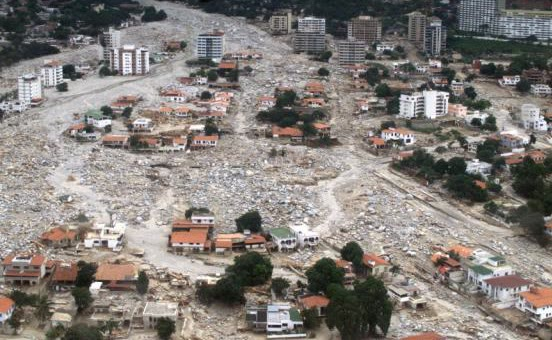
\includegraphics[width=0.62\linewidth]{images/book4/b2-28-caraballeda-debris-flow.jpg}
\par\smallskip{\small Endapan \omterm{def:b2:geological-hazards:slope}{aliran debris} di kipas Caraballeda, di pesisir Venezuela,
setelah badai Desember 1999: aliran-aliran itu meninggalkan alur utama dan mengubur kota di bawah
bongkah. (Foto: Lawson Smith dari Korps Zeni Angkatan Darat AS, domain publik.)}
\end{omfigure}
% ledger: photo:b2-28-caraballeda, vargas:caraballeda

\section{Tsunami}\label{sec:b2:geological-hazards:tsunamis}

Tsunami yang dibangkitkan oleh pengangkatan mendadak dasar laut memiliki panjang gelombang puluhan sampai ratusan
kilometer, jauh lebih besar daripada kedalaman samudra. Tsunami adalah gelombang panjang, dan kecepatannya hanya bergantung
pada kedalaman.

\begin{proposition}[Gelombang panjang]\label{prop:b2:geological-hazards:long-waves}
Gelombang gravitasi permukaan yang panjang gelombangnya jauh lebih besar daripada kedalaman air $h$ merambat dengan
$c = \sqrt{gh}$, berapa pun panjang gelombangnya. Di tempat gelombang itu bergerak perlahan ke air yang lebih dangkal tanpa
dipantulkan atau pecah, amplitudonya $A$ tumbuh sebagai $h^{-1/4}$.
\end{proposition}

\begin{proof}
Relasi dispersi memberikan kecepatan fase $c = \omega/k = \sqrt{(g/k)\tanh(kh)}$. Untuk gelombang
panjang $kh = 2\pi h/\lambda \ll 1$, dan $\tanh(kh) \approx kh$, sehingga $c = \sqrt{gh}$, tidak bergantung pada
$k$: gelombang panjang tidak terdispersi. Energi gelombang per satuan luas permukaan laut adalah $\frac12
\rho g A^2$, dan energi itu merambat dengan $c$. Jika tidak ada energi yang dipantulkan atau hilang, fluks $\frac12\rho g A^2
c$ melalui penampang mana pun sama di sepanjang lintasan: $A^2 \sqrt{h}$ konstan, dan $A \propto
h^{-1/4}$.
\end{proof}

Di atas air sedalam \qty{4000}{m} tsunami merambat dengan \qty{198}{m.s^{-1}}, \qty{713}{km/h}; di atas
\qty{5000}{m}, \qty{797}{km/h}, yaitu ``lebih dari 800 km/jam'' yang dikutip oleh layanan peringatan. Di dekat
pantai, di air sedalam \qty{10}{m}, tsunami melambat menjadi \qty{36}{km/h}; bagian depannya tersusul oleh air
di belakangnya, gelombang memendek dan menjadi curam, dan tingginya bertambah.
% ledger: nws:tsunami-speed

\begin{definition}[Rayapan tsunami]\label{def:b2:geological-hazards:tsunami}
Yang disebut \emph{rayapan tsunami}\index{rayapan tsunami} (\textit{run-up}) di suatu titik pantai adalah ketinggian, di atas
muka laut pada saat itu, dari tanah tertinggi yang dicapai air ke arah daratan di sana. Jarak horizontal
dari garis pantai ke titik itu adalah jarak genangan.
\end{definition}

Tim survei mengukur rayapan dari bekas air, garis rombakan, dan kerusakan setelah setiap tsunami. Basis
data tsunami global memuat \num{2177} pengamatan rayapan untuk tsunami Samudra Hindia
26 Desember 2004, yang dibangkitkan oleh gempa bumi bermagnitudo 9.1 di lepas pantai Sumatra, dengan tinggi air maksimum
\qty{50.9}{m}, dan \num{6429} untuk tsunami 11 Maret 2011 di lepas pantai Honshu, yang juga bermagnitudo 9.1,
dengan maksimum \qty{39.3}{m}. Keduanya menewaskan \num{227899} dan \num{18423} orang. Di Banda Aceh,
air mencapai pertengahan lantai kedua masjid di bawah ini.
% ledger: ncei:tsu-2004, ncei:tsu-2011, usgs:aceh-mosque

\begin{omfigure}
\centering
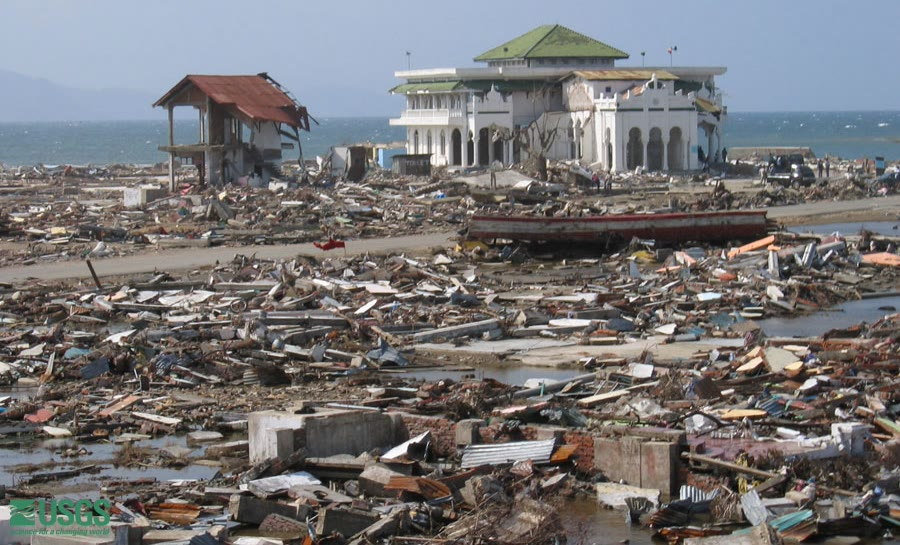
\includegraphics[width=0.62\linewidth]{images/book4/b2-28-aceh-mosque-tsunami.jpg}
\par\smallskip{\small Banda Aceh, Sumatra, pada 21 Januari 2005, setelah tsunami 26 Desember
2004: sebuah masjid berdiri di tengah puing-puing bangunan di sekitarnya. (Foto: U.S. Geological
Survey, domain publik.)}
\end{omfigure}
% ledger: photo:b2-28-aceh

\section{Banjir}\label{sec:b2:geological-hazards:floods}

\begin{definition}[Kurva frekuensi banjir]\label{def:b2:geological-hazards:flood}
Yang disebut \emph{kurva frekuensi banjir}\index{kurva frekuensi banjir} suatu sungai di suatu stasiun pengukur adalah
kurva debit puncak tahunan terhadap \omterm{def:b2:geological-hazards:return}{periode ulangnya}, atau terhadap \omterm{def:b2:geological-hazards:poisson}{probabilitas pelampauan}
tahunannya, yang dibangun dari rekaman puncak tahunan stasiun itu dan biasanya diperluas dengan suatu hukum
probabilitas hasil pencocokan.
\end{definition}

Rumus peringkat dari volume-volume sekolah menempatkan titik-titik kurva itu. Rumus itu punya alasan.

\begin{proposition}[Posisi plot Weibull]\label{prop:b2:geological-hazards:weibull}
Misalkan $n$ puncak tahunan saling bebas dan diambil dari distribusi kontinu yang sama, dan misalkan
$G(x)$ probabilitas bahwa puncak suatu tahun melampaui $x$. Puncak berperingkat $m$, yang dihitung dari
yang terbesar, memiliki \omterm{def:b2:geological-hazards:poisson}{probabilitas pelampauan} harapan $m/(n + 1)$, sehingga puncak itu diplot pada $T = (n +
1)/m$.
\end{proposition}

\begin{proof}
$U = G(X)$ seragam pada $[0, 1]$ untuk hukum yang kontinu, dan $G$ turun, sehingga
puncak terbesar ke-$m$ bersesuaian dengan nilai terkecil ke-$m$ dari $n$ peubah seragam yang saling bebas,
$U_{(m)}$. Kerapatannya adalah $f(u) = \frac{n!}{(m-1)!\,(n-m)!}u^{m-1}(1-u)^{n-m}$: satu dari $n$ nilai
berada di $u$, $m - 1$ di bawahnya, dan $n - m$ di atasnya. Dengan integral Beta $\int_0^1 u^{p}(1-u)^{q}\,\mathrm{d}u
= p!\,q!/(p + q + 1)!$,
\begin{equation*}
\mathbb{E}[U_{(m)}] = \frac{n!}{(m-1)!\,(n-m)!}\cdot\frac{m!\,(n-m)!}{(n+1)!} = \frac{m}{n+1}. \qedhere
\end{equation*}
\end{proof}

Puncak terbesar dalam rekaman 30 tahun dengan demikian diplot pada 31 tahun, dan tidak ada apa pun dalam rekaman itu yang menetapkan
banjir 100 tahun. Untuk mencapainya, puncak-puncak itu dicocokkan dengan suatu hukum nilai ekstrem, sering kali hukum Gumbel,
$\Pr(\text{puncak} \leq x) = \exp\bigl(-e^{-(x - u)/\alpha}\bigr)$, yang banjir $T$ tahunnya adalah $x_T = u
- \alpha\ln\bigl(-\ln(1 - 1/T)\bigr)$: garis lurus terhadap $-\ln(-\ln(1 - 1/T))$, yang diekstrapolasi
melampaui rekaman dengan risiko yang tumbuh seiring jaraknya.

\section{Pemantauan dan peringatan dini}\label{sec:b2:geological-hazards:warning}

\begin{definition}[Sistem peringatan dini]\label{def:b2:geological-hazards:warning}
Yang disebut \emph{sistem peringatan dini}\index{sistem peringatan dini} adalah sistem terpadu yang mencakup pemantauan
bahaya, prakiraan, penilaian risiko, komunikasi, dan kesiapsiagaan yang memungkinkan tindakan
tepat waktu sebelum suatu peristiwa berbahaya. Sistem itu menyatukan empat unsur: pengetahuan tentang risiko; deteksi,
pemantauan, dan prakiraan bahaya; penyebaran peringatan; dan kesiapsiagaan untuk
menanggapinya.
\end{definition}
% ledger: undrr:ews

Fisika menentukan berapa banyak waktu yang dapat diberikan setiap peringatan. Gelombang seismik tidak dapat didahului, tetapi gelombang S yang merusak
merambat dengan sekitar \qty{3.2}{km.s^{-1}} di kerak atas, dibandingkan dengan \qty{5.8}{km.s^{-1}} untuk
gelombang P: peringatan yang dihitung dari gelombang P pertama yang terekam di dekat episentrum mencapai suatu kota
sebelum gelombang S, sebesar $d(1/3.2 - 1/5.8) = \qty{0.14}{s}$ per kilometer jarak $d$, dikurangi
waktu untuk mendeteksi dan menghitung. Kota yang berjarak \qty{100}{km} memperoleh paling banyak \qty{14}{s}; di dekat sumber suatu
zona buta tidak memperoleh apa pun (\cref{exo:b2:geological-hazards:12}). Tsunami yang menyeberangi laut selebar \qty{100}{km}
dan sedalam \qty{2000}{m} memerlukan 12 menit; untuk menyeberangi suatu samudra diperlukan berjam-jam. Pada 2011, peringatan
Jepang dikeluarkan sekitar tiga menit setelah gempa bumi, tetapi dengan magnitudo yang diperkirakan terlalu rendah,
karena instrumen-instrumennya jenuh; peringatan itu diperbarui dengan data dari pelampung GPS lepas pantai sekitar 28 menit kemudian.
Perekam tekanan laut dalam, yang mengubah tekanan di dasar laut setiap 15 detik menjadi
tinggi permukaan laut, kini melaporkan tsunami yang lewat melalui satelit.
% ledger: data:prem, jma:warning, ndbc:dart
% values: 0.1401 s/km, 14.0 s at 100 km; 140 m/s over 2000 m, 11.9 min per 100 km (calc/ch28.py)

\begin{inthefield}[Mengamati lereng yang bergerak]
Pada lereng yang diketahui merayap, tim pemantau memasang instrumen yang mengukur variabel-variabel
persamaan lereng tak berhingga. Piezometer di dalam lubang bor merekam tekanan pori pada bidang gelincir;
pipa inklinometer, yang dibaca pada selang-selang kedalaman, menunjukkan di mana tanah melengkung dan seberapa cepat; stasiun
GNSS dan ekstensometer merekam gerakan permukaan; penakar hujan merekam pemicunya.
Tim-tim itu membandingkan gerakan dengan hujan dan tekanan air, musim demi musim, dan mencari
percepatan yang mendahului keruntuhan.
\end{inthefield}

\section*{Latihan}\label{sec:b2:geological-hazards:exercises}

Data untuk latihan, kecuali dinyatakan lain: $g = \qty{9.81}{m.s^{-2}}$; berat satuan air
\qty{9.81}{kN.m^{-3}}; GMPE \eqref{eq:b2:geological-hazards:gmpe} pada batuan ($G_B = G_C = 0$),
$\sigma = 0.230$; kecepatan P dan S di kerak atas 5.8 dan \qty{3.2}{km.s^{-1}}. Bulatkan sampai tiga
angka penting.
% ledger: bjf93:pga, data:prem

\begin{exercise}[$\star$]\label{exo:b2:geological-hazards:1}
Dengan model Poisson: (a) berapa probabilitas sedikitnya satu banjir 100 tahun dalam 30 tahun?
(b) Berapa probabilitas bahwa satu abad berlalu tanpa banjir 100 tahun? (c) Tentukan \omterm{def:b2:geological-hazards:return}{periode
ulang} gerakan dengan peluang pelampauan \qty{5}{\percent} dalam 50 tahun.
\end{exercise}

\begin{exercise}[$\star$]\label{exo:b2:geological-hazards:2}
Dua kota menghadapi guncangan kuat. Di kota A, guncangan itu terjadi dengan laju sekali dalam 200 tahun dan akan
menghancurkan \qty{2}{\percent} dari 5000 bangunannya; di kota B, sekali dalam 50 tahun, dan menghancurkan
\qty{10}{\percent} dari 800 bangunannya. (a) Tentukan banyaknya bangunan yang diharapkan hancur per
tahun di setiap kota. (b) Kota mana yang risikonya lebih besar, walaupun \omterm{def:b2:geological-hazards:risk}{keterpaparannya} lebih kecil? (c)
Faktor mana di antara ketiganya yang membuat perbedaan itu?
\end{exercise}

\begin{exercise}[$\star$]\label{exo:b2:geological-hazards:3}
(a) Tentukan kecepatan tsunami di atas kedalaman 4000, 200, dan \qty{10}{m}. (b) Berapa lama waktu yang diperlukannya
untuk menyeberangi samudra selebar \qty{1500}{km} yang sedalam \qty{4000}{m}? (c) Pada kedalaman berapa tsunami itu akan merambat dengan
\qty{800}{km/h}?
\end{exercise}

\begin{exercise}[$\star$]\label{exo:b2:geological-hazards:4}
Pasir kering tak berkohesi dengan $\varphi' = \ang{33}$ membentuk lereng yang panjang. (a) Tentukan \omterm{def:b2:geological-hazards:slope}{faktor
keamanannya} pada \ang{25}. (b) Berapa lereng tercuram yang dapat dibentuknya? (c) Lereng itu menjadi jenuh dengan
muka air tanah di permukaan dan rembesan yang sejajar dengannya, sehingga $r_u = \gamma_w\cos^2\beta/\gamma$
dengan $\gamma = \qty{20}{kN.m^{-3}}$. Tunjukkan bahwa $F = (1 - \gamma_w/\gamma)\tan\varphi'/\tan\beta$ dan
hitunglah nilainya pada \ang{25}.
\end{exercise}

\begin{exercise}[$\star\star$]\label{exo:b2:geological-hazards:5}
Katalog global memuat 696 gempa bumi bermagnitudo sedikitnya 7 dalam 50 tahun 1976--2025, dan
selang rata-rata di antaranya adalah 26.2 hari. (a) Tentukan laju tahunan rata-ratanya. (b) Dengan model
Poisson, berapa probabilitas bahwa 30 hari berlalu tanpa satu gempa pun? Bandingkan dengan fraksi teramati
selang yang lebih panjang daripada 30 hari, 0.304. (c) Berapa probabilitas sedikitnya satu gempa dalam
satu minggu tertentu?
\end{exercise}

\begin{exercise}[$\star\star$]\label{exo:b2:geological-hazards:6}
(a) Tentukan median PGA gempa bumi bermagnitudo 6.5 di batuan pada $d = 0$, 10, 30, dan
\qty{100}{km}. (b) Berapa nilainya pada \qty{10}{km} di lokasi kelas C? (c) Di antara nilai berapa
PGA di batuan pada \qty{10}{km} terletak dengan probabilitas sekitar \qty{68}{\percent}?
\end{exercise}

\begin{exercise}[$\star\star$]\label{exo:b2:geological-hazards:7}
Puncak tahunan suatu sungai selama 12 tahun, dalam \unit{m^3.s^{-1}}, adalah: 212, 148, 305, 176, 251, 133, 188,
420, 160, 229, 195, 268. (a) Berikan \omterm{def:b2:geological-hazards:return}{periode ulang} keempat puncak terbesar. (b) Perkirakan banjir 10
tahun dengan interpolasi linear dalam $\ln T$ di antara kedua puncak terbesar. (c) Mengapa rekaman ini tidak dapat mengatakan
apa pun yang dapat diandalkan tentang banjir 100 tahun?
\end{exercise}

\begin{exercise}[$\star\star$]\label{exo:b2:geological-hazards:8}
Pada suatu gunung api yang aktivitasnya meningkat, observatorium memperkirakan: peningkatan aktivitas magmatik 0.6; letusan jika magmatik 0.4;
eksplosif jika meletus 0.5; \omterm{def:b2:eruptive-styles:pdc}{aliran piroklastik} mencapai suatu lembah tertentu jika eksplosif 0.3. (a) Tentukan
probabilitas \omterm{def:b2:eruptive-styles:pdc}{aliran piroklastik} di lembah itu. (b) Tentukan probabilitas letusan, dan
probabilitas letusan tanpa aliran di lembah itu. (c) Data deformasi baru menaikkan probabilitas
letusan, jika peningkatan aktivitasnya magmatik, menjadi 0.7. Perbarui (a).
\end{exercise}

\begin{exercise}[$\star\star$]\label{exo:b2:geological-hazards:9}
Tanah kering dengan $c' = \qty{8}{kPa}$, $\varphi' = \ang{30}$, dan $\gamma = \qty{19}{kN.m^{-3}}$ terletak di atas
lereng \ang{35}. (a) Tentukan tebal $z_c$ saat $F = 1$. (b) Tentukan $F$ untuk lapisan
setebal \qty{2}{m}. (c) Lapisan yang sama menjadi jenuh, dengan muka air tanah di permukaan dan
$r_u = \gamma_w\cos^2\beta/\gamma$. Tentukan $F$.
\end{exercise}

\begin{exercise}[$\star\star\star$]\label{exo:b2:geological-hazards:10}
(a) Tunjukkan bahwa model Poisson tidak memiliki ingatan: probabilitas tidak adanya peristiwa dalam $[s, s + t]$, bila
tidak ada peristiwa dalam $[0, s]$, adalah $e^{-t/T}$, berapa pun $s$. (b) Suatu sesar memiliki \omterm{def:b2:geological-hazards:return}{periode ulang} 475 tahun untuk
gempa-gempa besarnya dan tidak mengalami satu pun selama 400 tahun. Menurut model itu, berapa probabilitas satu gempa
dalam 50 tahun mendatang? (c) Pantulan elastis dari volume Tahun 1 menyarankan bahwa probabilitas itu
seharusnya justru tumbuh seiring waktu sejak gempa terakhir. Asumsi model Poisson mana
yang dibantahnya, dan mengapa peta bahaya tetap memakai model itu untuk sumber areal?
\end{exercise}

\begin{exercise}[$\star\star\star$]\label{exo:b2:geological-hazards:11}
Tsunami dengan amplitudo \qty{0.5}{m} dan periode 20 menit menyeberangi samudra sedalam \qty{4000}{m}. (a)
Dengan memakai argumen fluks energi dari proposisi tentang gelombang panjang, tentukan amplitudonya di air sedalam \qty{10}{m}.
(b) Tentukan panjang gelombangnya pada kedua kedalaman. (c) Berikan dua alasan mengapa rayapan di pantai
dapat sangat berbeda dari perkiraan ini.
\end{exercise}

\begin{exercise}[$\star\star\star$]\label{exo:b2:geological-hazards:12}
Suatu \omterm{def:b2:geological-hazards:warning}{sistem peringatan dini} gempa bumi mengeluarkan peringatan 4 detik setelah gelombang P mencapai stasiunnya yang
terdekat dengan episentrum, yang berjarak \qty{10}{km}. Abaikan kedalaman sumber. (a) Kapan
peringatan itu dikeluarkan setelah gempa bumi? (b) Berapa detik sebelum gelombang S suatu kota yang berjarak \qty{50}{km}
dari episentrum menerimanya? Kota yang berjarak \qty{100}{km}? (c) Tentukan jari-jari zona buta, tempat
gelombang S tiba sebelum peringatan.
\end{exercise}

\begin{problem}[{Soal akhir pekan --- Sebuah kota di antara sesar dan lereng}]\label{pb:b2:geological-hazards:1}
Suatu kota di atas batuan terletak \qty{10}{km} dari suatu zona sumber; semua gempa buminya diambil pada
$d = \qty{10}{km}$. Perulangannya adalah $\log_{10} N(\geq M) = 4.0 - 1.0\,M$ per tahun untuk $M \geq 5$,
dipotong pada $M_{\max} = 7.5$. Guncangannya mengikuti GMPE \eqref{eq:b2:geological-hazards:gmpe}
dengan $\sigma = 0.230$. Di atas kota itu, suatu lapisan tanah setebal \qty{3}{m} terletak di atas lereng \ang{30},
dengan $\gamma = \qty{19}{kN.m^{-3}}$, $c' = \qty{4}{kPa}$, dan $\varphi' = \ang{34}$; air memiliki berat
satuan \qty{9.81}{kN.m^{-3}}. Bulatkan sampai tiga angka penting.

\noindent\textbf{Bagian I --- Perulangan.}
\begin{enumerate}
  \item Tentukan laju tahunan gempa bumi bermagnitudo sedikitnya 5, 6, dan 7, dengan mengabaikan
        pemotongan.
  \item Berikan \omterm{def:b2:geological-hazards:return}{periode ulang} yang bersesuaian.
  \item Dengan pemotongan, tentukan laju gempa bumi di atas 7.5, dan laju gempa bumi antara 7
        dan 7.5.
  \item Tentukan laju kelompok magnitudo 5--6 dan 6--7.
  \item Berapa probabilitas sedikitnya satu gempa bumi bermagnitudo 6 atau lebih dalam 50 tahun?
  \item Dan bermagnitudo 7 atau lebih?
\end{enumerate}

\noindent\textbf{Bagian II --- Gerakan tanah di kota.}
\begin{enumerate}[resume]
  \item Tentukan $r$, dan suku jarak $-0.778\log_{10} r$.
  \item Wakililah ketiga kelompok itu dengan magnitudo 5.5, 6.5, dan 7.25. Tentukan median
        $\log_{10}\mathrm{PGA}$ dan median PGA masing-masing.
  \item Tentukan PGA yang dilampaui dengan probabilitas \qty{16}{\percent} oleh gempa bermagnitudo 6.5.
  \item Berapa probabilitas bahwa gempa bermagnitudo 6.5 menghasilkan lebih dari \qty{0.3}{g}?
  \item Berapa median PGA gempa bumi terbesar yang mungkin?
\end{enumerate}

\noindent\textbf{Bagian III --- Kurva bahaya.}
\begin{enumerate}[resume]
  \item Tentukan laju tahunan pelampauan \qty{0.2}{g}, yang dijumlahkan atas ketiga kelompok.
  \item Hal yang sama untuk \qty{0.3}{g}.
  \item Hal yang sama untuk \qty{0.4}{g}.
  \item Laju tahunan berapa yang bersesuaian dengan \qty{10}{\percent} dalam 50 tahun?
  \item Di antara dua tingkat yang mana dari ketiga tingkat itu laju tersebut jatuh?
  \item Dengan interpolasi linear dalam $\ln\lambda$ terhadap $\ln a$, tentukan PGA dengan
        peluang pelampauan \qty{10}{\percent} dalam 50 tahun.
  \item Kelompok mana yang paling banyak menyumbang pada laju di \qty{0.3}{g}? Berikan komentar, dengan memakai jawaban
        pertanyaan~11.
\end{enumerate}

\noindent\textbf{Bagian IV --- Lereng di atas kota.}
\begin{enumerate}[resume]
  \item Tentukan \omterm{def:b2:geological-hazards:slope}{faktor keamanan} lereng yang kering.
  \item Tentukan \omterm{def:b2:geological-hazards:slope}{faktor keamanannya} bila lapisan itu jenuh, dengan muka air tanah di permukaan ($r_u =
        \gamma_w\cos^2\beta/\gamma$).
  \item Sampai fraksi berapa dari tebal lapisan muka air tanah dapat naik sebelum lereng itu runtuh?
  \item Dalam analisis pseudostatis (diterima tanpa bukti), guncangan menambahkan gaya horizontal $kW$. Tentukan
        $k$ kritis lereng yang kering, saat $F = 1$.
  \item Dengan mengambil $k$ sama dengan PGA dalam satuan $g$, magnitudo mana yang menghasilkan nilai kritis itu sebagai
        mediannya di kota? Bandingkan dengan jawaban pertanyaan~17.
  \item Sebagai ringkasan: berapa \omterm{def:b2:geological-hazards:psha}{percepatan tanah puncak} dengan peluang \qty{10}{\percent} untuk
        dilampaui dalam 50 tahun di kota itu?
\end{enumerate}
\end{problem}
